\setcounter{chapter}{6-1}

\chapter{Neural Networks 1.5 - Back-Propagation and Training}


\setcounter{section}{4}
%\pagebreak
%%%%%%%%%%%%%%%%%%%%%%%%%%%%%%%%%%%%%%%%%%%%%%%%%%%%%%%%%%%%%%%%%%%%%%%%%%%%%  
\section{Error back-propagation }

    We have a complete neural network: a \textbf{model} we can use to make predictions or calculations.
    
    Now, our mission is to \textbf{improve} this neural network: even if our hypothesis class is good, we still have to \textbf{find} the hypotheses that are useful for our problem.
    
    As usual, we will start out with \textbf{randomized} values for our weights and biases: this \textbf{initial} neural network will not be useful for anything in particular, but that's why we need to improve it.
        \note{We randomize them because otherwise, if our initialization is \\$w_i=0$, we get $$w^T x+w_0=0$$ no matter what input $x$ we have.}
    
    For such a complex problem, we definitely can't find an explicit solution, like we did for ridge regression. Instead, we will have to rely on \textbf{gradient descent}.\\
    
    \begin{concept}
        \vocab{Neural networks} are typically optimized using \purp{gradient descent}.
    \end{concept}
    
    \secdiv
    
    \subsection{Review: Gradient Descent}
    
        What does it really mean to do gradient descent on our \textbf{network}? Let's remind ourselves of how gradient descent works, and then \textbf{build} up to a network.
        
        \begin{concept}
            \vocab{Gradient descent} works based on the following reasoning:
        
            \begin{itemize}
                \item We have a function we want to \purp{minimize}: our loss function $\loss$, which tells us how \gren{badly} we're doing.
                    \begin{itemize}
                        \item We want to perform "less badly".
                    \end{itemize}
                    
                \boxdiv
                    
                \item Our main tool for \purp{improving} $\loss$ is to alter $\theta$ and $\theta_0$.
                    \begin{itemize}
                        \item These are our \gren{parameters}: we're adjusting our model.
                    \end{itemize}
                    
                
                    
                \item The \purp{gradient} is our main tool: $\pderiv{B}{A}$ tells you the direction to \gren{change} $A$ in order to \redd{increase} $B$.
                
                \boxdiv
                
                \item We want to \gren{change} $\theta$ to \redd{decrease} $\loss$. Thus, we move in the direction of 
                    
                    \begin{equation}
                        \Delta \theta = -\eta \pderiv{\loss}{\theta}
                    \end{equation}
                    
                    \begin{itemize}
                        \item Remember that $\eta$ is our \vocab{step size}: we can take bigger or smaller steps in each direction.
                    \end{itemize}
                    
                \boxdiv
                    
                \item We take steps $\Delta \theta$ (and $\Delta \theta_0$) until we are satisfied with $\loss$, or it \gren{stops} improving.
            \end{itemize}
            
        \end{concept}
        
    \secdiv  
        
    \subsection{Review: Gradient Descent with LLCs}
    
        Let's start with a familiar example: \textbf{LLCs}.
        
        Our LLC model uses the following equations:
            \note{We'll use $w$ instead of $\theta$.}
        
        \begin{equation}
            \red{
                z(x) = w^T x + w_0  
            }
            \qquad \qquad
            \blu{
                g(z) = \sigma(z) = \frac{1}{1+e^{-z}}
            }
        \end{equation}
        
        \begin{equation}
            \pur{
                \loss(g,y) = y\log(g) + (1-y)\log(1-g)
            }
        \end{equation}
        
        Our goal is to minimize $\loss$ by adjusting $\theta$ and $\theta_0$.
        
        So, we want 
        
        \begin{equation}
            \pderiv {\pur{\loss}} {w} 
            \qquad \text{and} \qquad 
            \pderiv {\pur{\loss}} {w_0}
        \end{equation}
        
        We did this by using the \textbf{chain rule}:
            \note{We'll focus on $w$, but the same goes for $w_0$.}
        
        \begin{equation}
            \pderiv {\pur{\loss}} {w} 
            =
                \overbrace{
                \pderiv {\pur{\loss}} {\blu{g}} 
                    \cmul
                \pderiv {\blu{g}}     {w}
            }^{\loss(g)}
        \end{equation}
        
        We can break it up further using \textbf{repeated} chain rules:
        
        \begin{equation}
            \pderiv {\pur{\loss}} {w} 
            =%Goal: overlapping braces.
            \mathrlap{ %\mathrlap allows brace to overlap with the next section
                \overbrace{ %Create brace
                    \phantom{ %Create phantom text so our brace is the right size
                        \pderiv {\pur{\loss}} {\blu{g}} 
                            \cmul
                        \pderiv {\blu{g}}     {\red{z}}
                    }
                }^{\loss(g)} %Brace superscript
            }
            \pderiv {\pur{\loss}} {\blu{g}} 
                \cmul
            \underbrace{
                \pderiv {\blu{g}}     {\red{z}}
                    \cmul
                \pderiv {\red{z}}     {w}
            }_{g(z)}
        \end{equation}
        
        Plugging in our derivatives, we get:
        
        \begin{equation}
            \pderiv {\pur{\loss}} {w}
            =
            \overbrace{
                -
                \Big(
                    \frac{ \org{y} } { \blu{\sigma} } 
                    -
                    \frac{ 1-\org{y} } { 1 - \blu{\sigma} }
                \Big)
            }^{ \pderivslash{\loss}{g} }
            \cdot
            \overbrace{
                \blu{\sigma} (1-\blu{\sigma})
            }^{ \pderivslash{g}{z} }
            \cdot 
            \overbrace{
            x
            }^{ \pderivslash{z}{w} }
        \end{equation}

        \begin{concept}
            The \vocab{chain rule} allows us to take the gradient of \purp{nested functions}, where each function is the \gren{input} to the next one.
            
            Another way to say this is that one function \vocab{feeds into} the next.
        \end{concept}
            
            \note{If you aren't familiar with "nested" functions, consider this example:\\
            \phantom{ }\\
            If you have functions $f(x)$ and $g(x)$, then $g(f(x))$ is the \textbf{nested} combination, where the output of $f$ is the input of $g$.}
    
    \secdiv
    
    \subsection{Review: LLC as Neuron}
    
        Remember that we can represent our LLC as a \textbf{neuron}: this could give us the first idea for how to train our \textbf{neural network}!
        
        \begin{figure}[H]
            \centering
            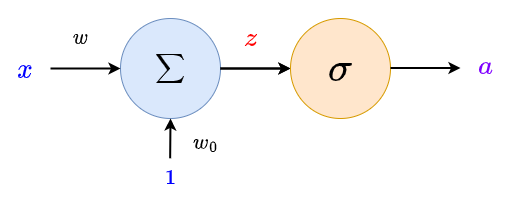
\includegraphics[width=80mm,scale=0.4]{images/nn_1_5_images/llc_as_neuron.png}
        \end{figure}
        
        As usual, our first unit $\sum$ is our \textbf{linear} component. The output is $z$, nothing different from before with LLC.
            \note{Remember that $x$ is a whole vector of values, which we've condensed into one variable.}
        
        The \textbf{output} of $\sigma$, which we wrote before as $g$, is now $a$.
        
        Something we neglected before: this diagram is \textbf{missing} the \textbf{loss function}. Let's create a small unit for that. 
        
        $\loss(a,y)$ has \textbf{two} inputs: our predicted value $a$, and the correct value $y$. 
        
        \begin{figure}[H]
            \centering
            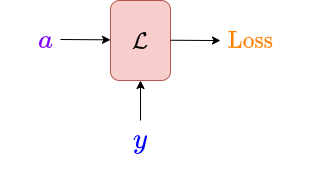
\includegraphics[width=60mm,scale=0.4]{images/nn_1_5_images/loss_unit.png}
            \caption*{We have two inputs to our loss function.}
        \end{figure}
        
        We \textbf{combine} these into a single unit to get:
        
        \begin{figure}[H]
            \centering
            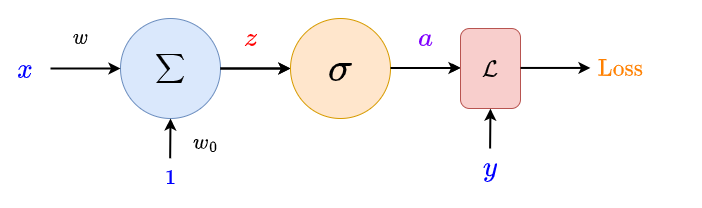
\includegraphics[width=90mm,scale=0.4]{images/nn_1_5_images/llc_as_neuron_loss.png}
        \end{figure}
        
        Our full unit!
        
    \secdiv
    
    \subsection{LLC Forward-Pass}
    
        Now, we can do gradient descent like before. We want to get the effect our \textbf{weight} has on our \textbf{loss}.
        
        But, this time, we'll pair it with a \textbf{visual} that is helpful for understanding how we \textbf{train} neural networks. 
        
        First, one important consideration:
        
        As we saw above, the \textbf{gradient} we get might rely on $z$, $a$, or $\loss(a,y)$. So, before we do anything, we have to \textbf{compute} these values.
        
        Each step \textbf{depends} on the last: this is what the \textbf{forward} arrows represent. We call this a \textbf{forward pass} on our neural network.\\
        
        \begin{definition}
            A \vocab{forward pass} of a neural network is the process of sending information "\gren{forward}" through the neural network, starting from the \purp{input}.
            
            This means the \purp{input} is fed into the \gren{first} layer, and that output is fed into the \gren{next} layer, and so on, until we reach our \purp{final} result and \purp{loss}.
        \end{definition}
        
        \miniex If we had 
        
        \begin{itemize}
            \item $\blu{f}(\red{x}) = \red{x}+2$
            
            \item $\org{g}(\blu{f}) = 3\blu{f}$
            
            \item $h(\org{g}) = \sin(\org{g})$
        \end{itemize}
        
        Then, a forward pass with the input $x=10$ would have us go function-by-function:
        
        \begin{itemize}
            \item $\blu{f}(\red{10}) = \red{10}+2$
            
            \item $\org{g}(\blu{f}) = 3 \cdot \blu{12}$
            
            \item $h(\org{g}) = \sin(\org{36})$
        \end{itemize}
        
        So, by "forward", we mean that we apply each function, one after another.
        
        In our case, this means computing $z$, $a$, and $\loss(a,y)$.
        
    \secdiv
    
    \subsection{LLC Back-propagation}
    
        Now that we have all of our values, we can get our gradient. Let's \textbf{visualize} this process.
        
        \begin{figure}[H]
            \centering
            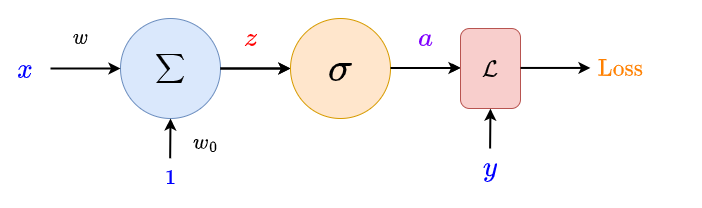
\includegraphics[width=90mm,scale=0.4]{images/nn_1_5_images/llc_as_neuron_loss.png}
        \end{figure}
        
        We want to link $\loss$ to $w$. In order to do that, we need to \textbf{connect} each thing in between.
        
        This lets us \textbf{combine} lots of simple \textbf{links} to get our more complicated result.
            \note{We can also call this "chaining together" lots of derivatives.}
            
        Loss is what we really care about. So, what is the loss directly \textbf{connected} to? The \textbf{activation}, $a$.
        
        \begin{figure}[H]
            \centering
            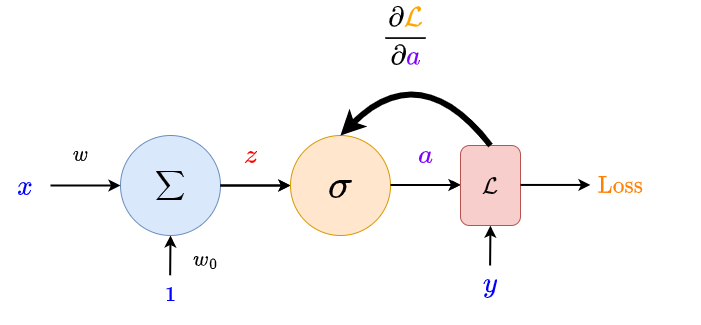
\includegraphics[width=90mm,scale=0.4]{images/nn_1_5_images/llc_backprop_1.png}
        \end{figure}
        
        So, our $\sigma$ unit has information about the derivative that comes after it: the \textbf{loss} derivative
        
        \begin{equation}
            \overbrace{
                \pderiv {\pur{\loss}} {\blu{a}} 
            }^{\text{Loss unit}} 
        \end{equation}
        
        And what is that connected to? The \textbf{pre-activation} $z$:
        
        \begin{figure}[H]
            \centering
            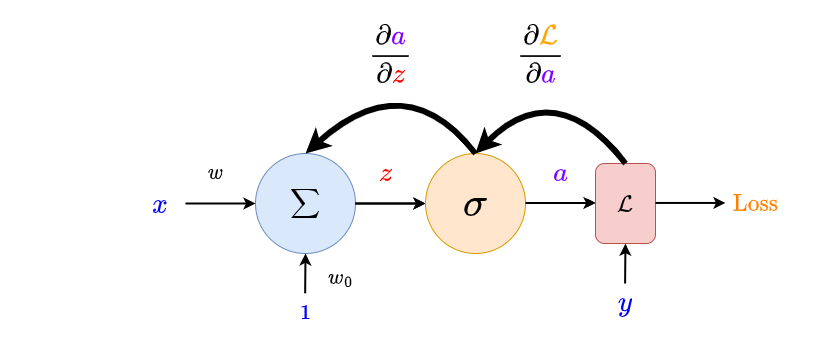
\includegraphics[width=100mm,scale=0.4]{images/nn_1_5_images/llc_backprop_2.png}
        \end{figure}
        
        Now, our $\sum$ unit has information about both the \textbf{loss} derivative and the $\sigma$ derivative:
        
        \begin{equation}
            \overbrace{
                \pderiv {\pur{\loss}} {\blu{a}} 
            }^{\text{Loss unit}}
            \cmul
            \overbrace{
                \pderiv {\blu{a}}     {\red{z}}
            }^{\text{Activation function}}
        \end{equation}
       
        
        And finally, we've reached $w$:
        
        \begin{figure}[H]
            \centering
            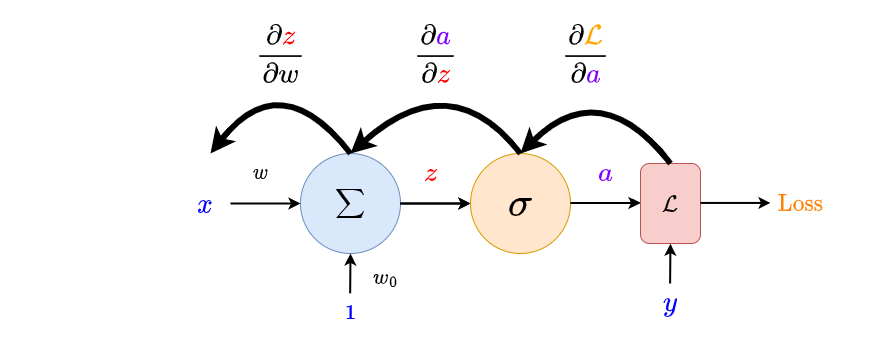
\includegraphics[width=110mm,scale=0.4]{images/nn_1_5_images/llc_backprop_3.png}
        \end{figure}
        
        And, we built our chain rule! This contains the \textbf{information} of the derivatives from \textbf{every} unit.
        
        \begin{equation}
            \pderiv {\pur{\loss}} {w} 
            =
            \overbrace{
                \pderiv {\pur{\loss}} {\blu{a}} 
            }^{\text{Loss unit}}
            \cmul
            \overbrace{
                \pderiv {\blu{a}}     {\red{z}}
            }^{\text{Activation}}
                \cmul
            \overbrace{
                \pderiv {\red{z}}     {w}
            }^{\text{Linear subunit}}
        \end{equation}
        
        Moving backwards like this is called \textbf{back-propagation}.\\
        
        \begin{definition}
            \vocab{Back-propagation} is the process of moving "\gren{backwards}" through your network, starting at the \purp{loss} and moving back layer-by-layer, and gathering terms in your \purp{chain rule}.
            
            We call it "\purp{propagation}" because we send backwards the \gren{terms} of our chain rule about later derivatives.
            
            An \gren{earlier} unit (closer to the "left") has all of the \purp{derivatives} that come after (to the "right" of) it, along with its own term.
        \end{definition}
        
    \secdiv
    
    \subsection{Summary of neural network gradient descent: a high-level view}
    
        So, with just this, we have built up the basic idea of how we \textbf{train} our model: now that we have the gradient, we can do \textbf{gradient descent} like we normally do!
            \note{This summary covers some things we haven't fully discussed. We'll continue digging into the topic!}\\
        
        \begin{concept}
            We can do \vocab{gradient descent} on a \vocab{neural network} using the ideas we've built up:
            
            \boxdiv
            
            \begin{itemize}
                \item Do a \vocab{forward pass}, where we compute the value of each \gren{unit} in our model, passing the information \purp{forward} - each layer's \textbf{output} is the next layer's \textbf{input}.
                    \begin{itemize}
                        \item We finish by getting the \purp{loss}.
                    \end{itemize}
                    
            \boxdiv
                    
                \item Do \vocab{back-propagation}: build up a \purp{chain rule}, starting at the \purp{loss} function, and get each unit's \gren{derivative} in \purp{reverse order}.
                    \begin{itemize}
                        \item \purp{Reverse} order: if you have 3 layers, you want to get the 3rd layer's \gren{derivatives}, then the 2nd layer, then the 1st.
                        
                        \item \purp{Each weight} vector has its own \gren{gradient}: we'll deal with this later, but we need to calculate one for each of them.
                    \end{itemize}
                    
            \boxdiv
                
                \item Use your chain rule to get the \purp{gradient} $\pderiv{\loss}{w}$ for your \gren{weight} vector(s). Take a \vocab{gradient descent} step.
                
                \item \vocab{Repeat} until satisfied, or your model \purp{converges}.
            \end{itemize}
        \end{concept}
        
    \secdiv
    
    \subsection{A two-neuron network: starting backprop}
        
        Above, we mention "\textbf{each} layer": we'll now transition to a \textbf{two-neuron} system, so we have "two layers". Then, we'll build up to many layers.
        
        Remember, though, that the \textbf{ideas} represented here are just extensions of what we did \textbf{above}.
        
        Let's get a look at our \textbf{two-neuron} system, now with our \textbf{loss} unit:
        
        \begin{figure}[H]
            \centering
            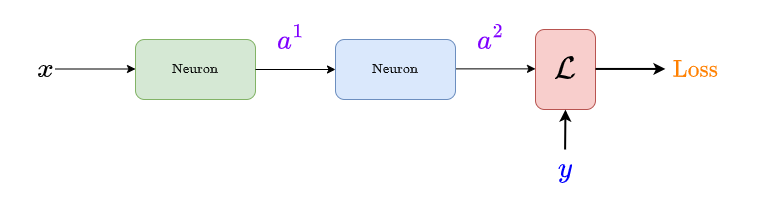
\includegraphics[width=140mm,scale=0.4]{images/nn_1_5_images/two_neurons_bp.png}
        \end{figure}
        
        And unpack it:
        
        \begin{figure}[H]
            \centering
            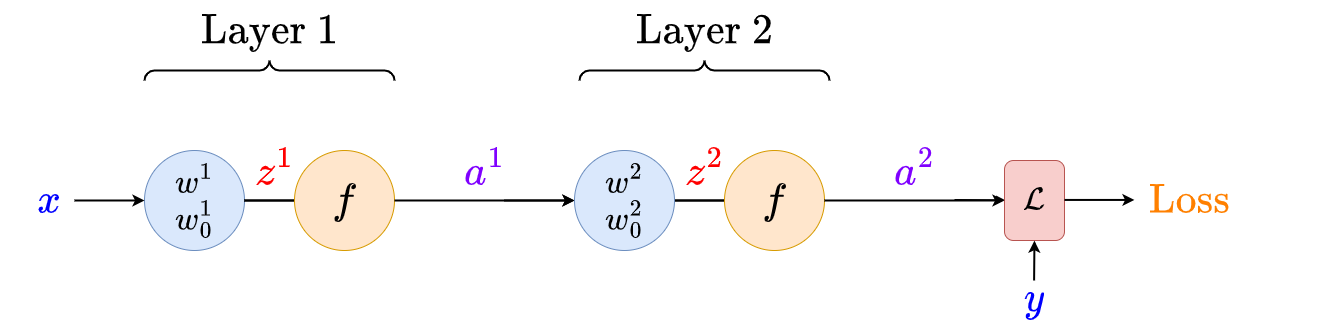
\includegraphics[width=140mm,scale=0.4]{images/nn_1_5_images/two_neurons_inside_bp.png}
        \end{figure}
        
        We want to do \textbf{back-propagation} like we did before. This time, we have \textbf{two} different layers of weights: $w^1$ and $w^2$. Does this cause any problems?
        
        It turns out, it doesn't! We mentioned in the first part of chapter 7 that we can treat the \textbf{output} of the \textbf{first} layer $a^1$ as the same as if it were an \textbf{input} $x$.
            \note{This is one of the biggest benefits of neural network layers!}
            
        \begin{figure}[H]
            \centering
            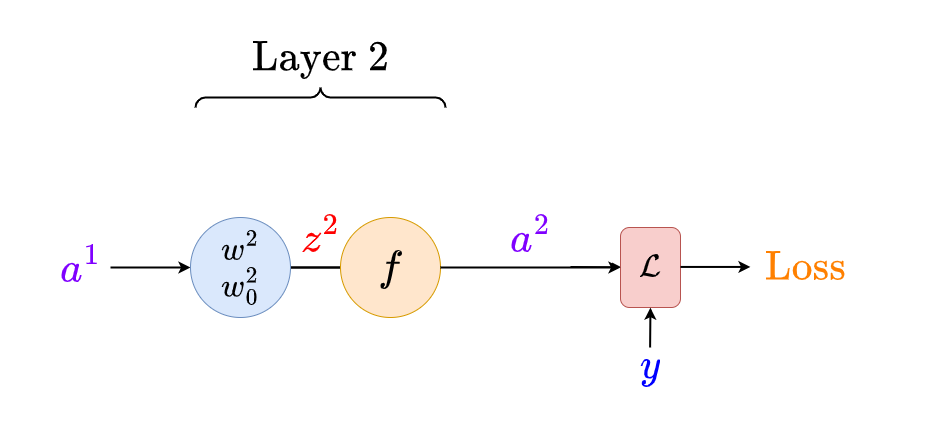
\includegraphics[width=90mm,scale=0.4]{images/nn_1_5_images/layer2_bp.png}
        \end{figure}
        
        Now, we can do backprop safely.
            \note{"Backprop" is a common shortening of "back-propagation".}
        
        \begin{figure}[H]
            \centering
            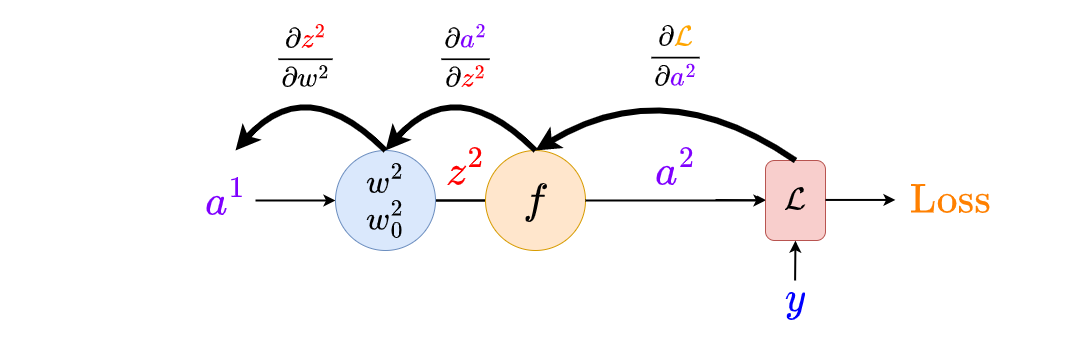
\includegraphics[width=120mm,scale=0.4]{images/nn_1_5_images/layer2_bp1.png}
        \end{figure}
        
        We can get:
        
        \begin{equation}
            \pderiv {\pur{\loss}} {w^2} 
            =
            \overbrace{
                \pderiv {\pur{\loss}} {\blu{a^2}} 
            }^{\text{Loss unit}}
            \cmul
            \overbrace{
                \pderiv {\blu{a^2}}     {\red{z^2}}
            }^{\text{Activation}}
                \cmul
            \overbrace{
                \pderiv {\red{z^2}}     {w^2}
            }^{\text{Linear}}
        \end{equation}
        
        The same format as for our \textbf{one-neuron} system! We now have a gradient we can update for our \textbf{second} weight vector.
        
        But what about our \textbf{first} weight vector?
        
    \secdiv
    
    \subsection{Continuing backprop: One more problem}
    
        We need to continue further to reach our \textbf{earlier} weights: this is why we have to work \textbf{backward}.\\
        
        \begin{concept}
            We work \purp{backward} in \vocab{back-propagation} because every layer after the \gren{current} one \purp{affects} the gradient.
            
            Our current layer \gren{feeds} into the next layer, which feeds into the layer after that, and so on. So this layer affects \purp{every} later layer, which then affect the loss.
            
            So, to see the effect on the \purp{output}, we have to \gren{start} from the \purp{loss}, and get every layer \purp{between} it and our weight vector.
        \end{concept}
            
            \note{Remember that when we say "$f$ feeds into $g$", we mean that the output of $f$ is the input to $g$.}
            
        \phantom{ }
            
        \begin{figure}[H]
            \centering
            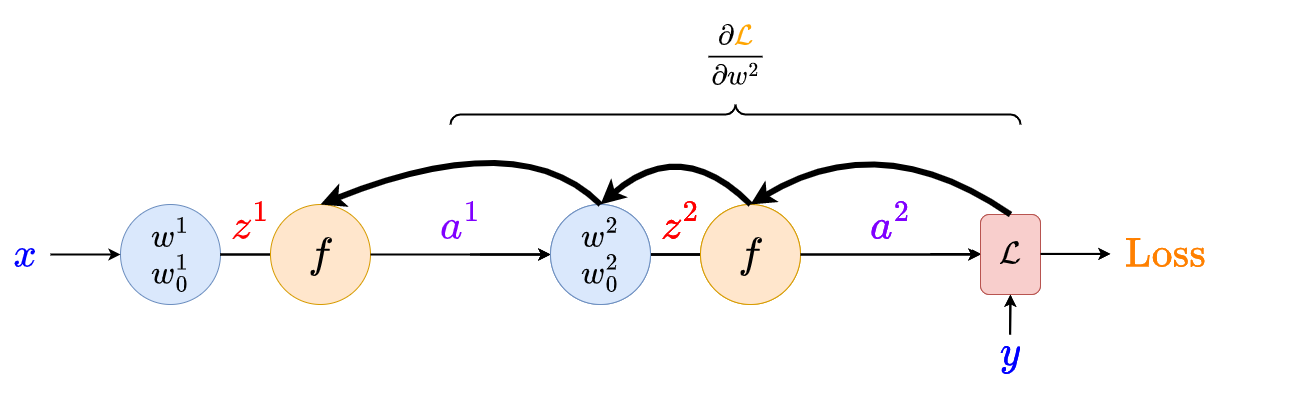
\includegraphics[width=120mm,scale=0.4]{images/nn_1_5_images/two_neurons_inside_bp2.png}
        \end{figure}
            
        We have one problem, though: 
        
        We just gathered the derivative $\pderivslash {\pur{\loss}} {w^2} $. If we wanted to continue the chain rule, we would expect to add more terms, like:
            \note{Since our current derivative includes $w^2$, we would continue it with a $w^2$ in the 
            "top" of a derivative, 
            $$\pderiv{\pur{\loss}}{w^2} \pderiv{w^2}{r}$$
            We're not sure what "$r$" is yet.}
        
        \begin{equation}
            \pderiv{w^2}{a^1}
        \end{equation}
        
        The problem is, what is $w^2$? It's a vector of constants.
        
        \begin{equation}
            w^2 = 
            \begin{bmatrix}
                    w_1^2 \\ w_2^2 \\ \vdots \\ w_n^2
            \end{bmatrix}
            ,
            \qquad
            \qquad
            \text{Not a function of $a^1$!}
        \end{equation}
        
        That derivative above is going to be \textbf{zero}! In other words, $w^2$ isn't really the \textbf{input} to $z^2$: it's a \textbf{parameter}.
            \note{We were building our chain rule by combining inputs with outputs: that's what links two layers together.\\
            \phantom{ }\\
            So, it should make sense that using something like $w$ (that doesn't link two layers) prevents us from making a longer chain rule.}
            
        So, we can't end our derivative with $w^2$. Instead, we have to use something else. $z^2$'s real input is $a^1$, so let's go directly to that!
        
        \begin{figure}[H]
            \centering
            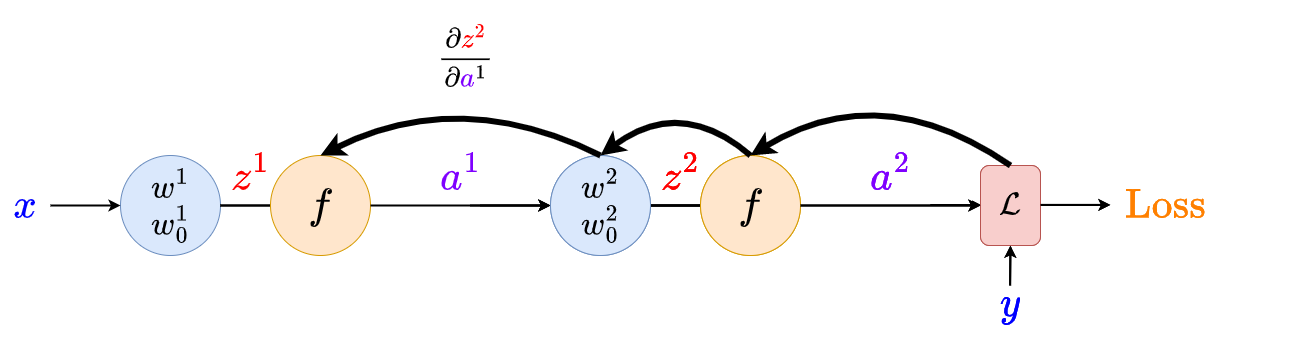
\includegraphics[width=120mm,scale=0.4]{images/nn_1_5_images/two_neurons_inside_bp3.png}
            \caption*{Using this allows us to move from layer 2 to layer 1.}
        \end{figure}
        
        Now, we have our new chain rule:
        
        \begin{equation}
            \pderiv {\pur{\loss}} {a^1} 
            =
            \overbrace{
                \pderiv {\pur{\loss}} {\blu{a^2}} 
                    \cmul
                \pderiv {\blu{a^2}}   {\red{z^2}}
            }^{\text{Other terms} } 
                \cmul
            \overbrace{
                \pderiv {\red{z^2}}   {a^1}
            }^{\text{Link Layers}}
        \end{equation}
        
        \begin{concept}
            For our \vocab{weight gradient} in layer $l$, we have to end our \purp{chain rule} with
            
            \begin{equation*}
                \pderiv {\red{z^\ell}}   {w^\ell}
            \end{equation*}
            
            So we can get 
            
            \begin{equation*}
                \pderiv {\pur{\loss}} {w^\ell} 
                =
                \overbrace{
                    \pderiv {\pur{\loss}} {\red{z^\ell}} 
                }^{\text{Other terms} }
                \cmul  
                \overbrace{
                    \pderiv {\red{z^\ell}}   {w^\ell}
                }^{\text{Get weight grad}}
            \end{equation*}
            
            However, because $w^l$ is not the \textbf{input} of layer $l$, we can't use it to find the gradient of \gren{earlier layers}.
            
            Instead, we use 
            
            \begin{equation}
                \pderiv {\red{z^\ell}}   {a^{\ell-1}}
            \end{equation}
            
            To "\purp{link together}" two different layers $\ell$ and $\ell-1$ in a \gren{chain rule}.
        \end{concept}
        
            \note{In this section, we compressed lots of derivatives into 
            $$\pderiv {\pur{\loss}} {\red{z^\ell}}$$
            Don't let this alarm you, this just hides our long chain of derivatives!}
            
    \secdiv
    
    \subsection{Finishing two-neuron backprop}
    
        Now that we have safely connected our layers, we can do the rest of our gradient. First, let's lump together everything we did before:
        
        \begin{figure}[H]
            \centering
            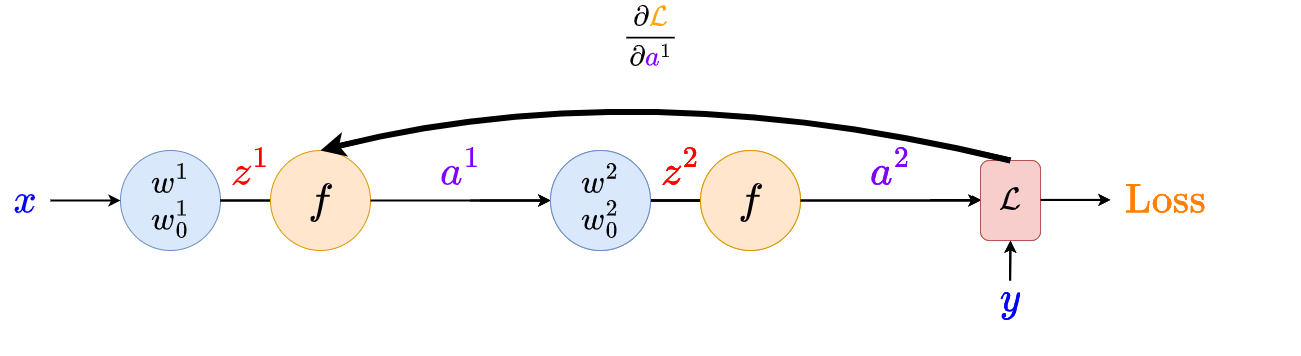
\includegraphics[width=120mm,scale=0.4]{images/nn_1_5_images/two_neurons_inside_bp4.png}
            \caption*{All the info we need is stored in this derivative: it can be written out using our friendly chain rule from earlier.}
        \end{figure}
        
        Now, we can add our remaining terms. It's the same as before: we want to look at the pre-activation
        
        \begin{figure}[H]
            \centering
            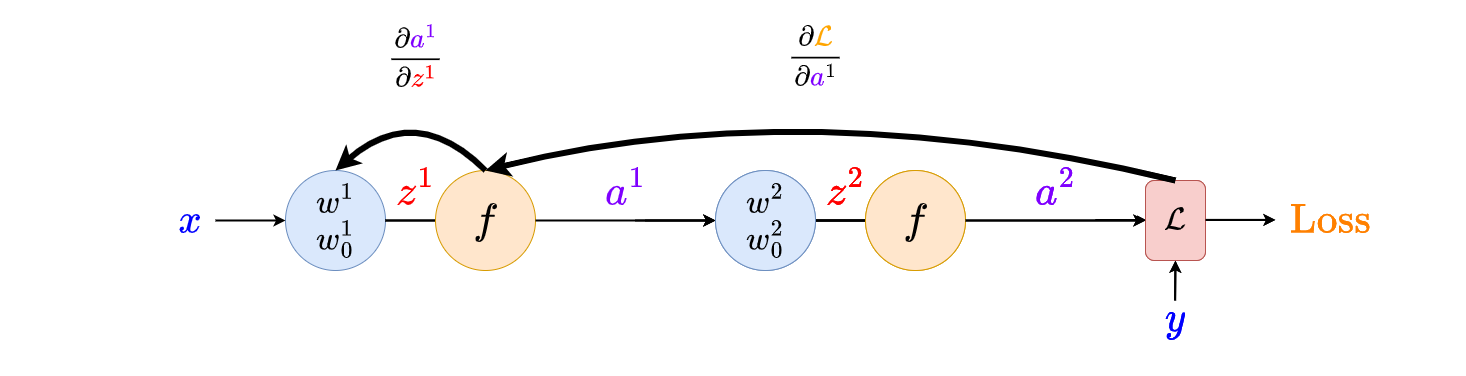
\includegraphics[width=120mm,scale=0.4]{images/nn_1_5_images/two_neurons_inside_bp5.png}
        \end{figure}
        
        And finally, our input:
        
        \begin{figure}[H]
            \centering
            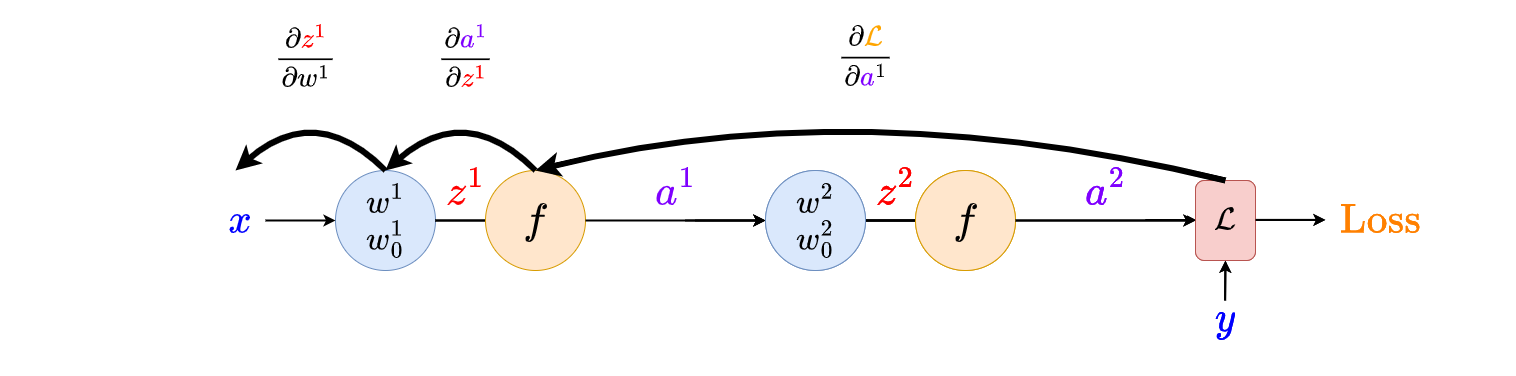
\includegraphics[width=120mm,scale=0.4]{images/nn_1_5_images/two_neurons_inside_bp6.png}
        \end{figure}
        
        We can get our second chain rule
        
        \begin{equation}
            \pderiv {\pur{\loss}} {w^1} 
            =
            \overbrace{
                \pderiv {\pur{\loss}} {\blu{a^1}} 
            }^{\text{Other layers}}
            \cmul
            \overbrace{
                \pderiv {\blu{a^1}}   {\red{z^1}}
                \cmul
                \pderiv {\red{z^1}}   {w^1}
            }^{\text{Layer 1}}
        \end{equation}
        
        Which, in reality, looks much bigger:
        
        \begin{equation}
            \pderiv {\pur{\loss}} {w^1} 
            =
            \overbrace{
                \Bigg(
                    \pderiv {\pur{\loss}} {\blu{a^2}} 
                \Bigg)
            }^{\text{Loss unit}}
            \cmul
            \overbrace{
                \Bigg(
                    \pderiv {\blu{a^2}}   {\red{z^2}}
                        \cmul
                    \pderiv {\red{z^2}}   {a^1}
                \Bigg) 
            }^{\text{Layer 2}}
            \cmul
            \overbrace{
                \Bigg(
                    \pderiv {\blu{a^1}}   {\red{z^1}}
                        \cmul
                    \pderiv {\red{z^1}}   {w^1}
                \Bigg)
            }^{\text{Layer 1}}
        \end{equation}
        
        We see a clear \textbf{pattern} here! In fact, this is the procedure we'll use for a neural network with \textbf{any} number of layers.\\
        
        \begin{concept}
            We can get all of our \vocab{weight gradients} by repeatedly appending to the \purp{chain rule}.
            
            For each layer, we multiply by
            
            \begin{equation*}
                \overbrace{
                    \pderiv {\blu{a^\ell}} {\red{z^\ell}}
                }^{\text{Within layer}}
                    \cmul
                \overbrace{
                    \pderiv {\red{z^\ell}} {w^\ell}
                }^{\text{Get weight grad}}
            \end{equation*}
            
            To get the \purp{weight gradient} $\pderivslash{ \pur{\loss} }{w^\ell}$.
            
            If we want to \gren{extend} to the next layer, we \red{instead} multiply by
            
            \begin{equation*}
                \overbrace{
                    \pderiv {\blu{a^\ell}} {\red{z^\ell}}
                }^{\text{Within layer}}
                    \cmul
                \overbrace{
                    \pderiv {\red{z^\ell}} {a^{\ell-1}}
                }^{\text{Link layers}}
            \end{equation*}
            
        \end{concept}
        
    \secdiv
    
    \subsection{Many layers: Doing back-propagation}
    
        Now, we'll consider the case of many possible layers.
            \note{To make it more readable, we'll use boxes instead of circles for units.}
            
        \phantom{ }
            
        \begin{figure}[H]
            \centering
            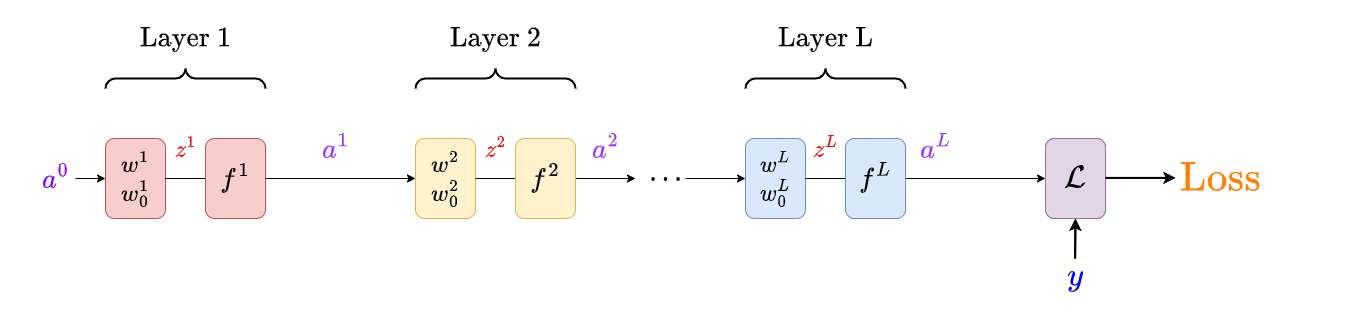
\includegraphics[width=180mm,scale=0.4]{images/nn_1_5_images/network_bp.png}
        \end{figure}
        
        This may look intimidating, but we already have all the tools we need to handle this problem.
        
        Our goal is to get a \textbf{gradient} for each of our \textbf{weight} vectors $w^\ell$, so we can do gradient descent and \textbf{improve} our model.
        
        According to our above analysis in Concept 9, we need only a few steps to get all of our gradients.
        
        \begin{concept}
            In order to do \vocab{back-propagation}, we have to build up our \vocab{chain rule} for each weight gradient.
            
            \begin{itemize}
                \item We start our chain rule with one term shared by every gradient: 
                    \begin{equation*}
                        \overbrace{
                            \pderiv {\pur{\loss}} {\blu{a^L}} 
                        }^{\text{Loss unit}}
                    \end{equation*}
            \end{itemize}
            
            Then, we follow these two steps until we run out of layers:
            \begin{itemize}
                \item We're at layer $\ell$. We want to get the \purp{weight gradient} for this layer. We get this by \gren{multiplying} our chain rule by
                
                    \begin{equation*}
                        \overbrace{
                            \pderiv {\blu{a^\ell}} {\red{z^\ell}}
                        }^{\text{Within layer}}
                            \cmul
                        \overbrace{
                            \pderiv {\red{z^\ell}} {w^\ell}
                        }^{\text{Get weight grad}}
                    \end{equation*}
                    
                    We \red{exclude} this term for any other gradients we want.
                
                \item If we aren't at layer 1, there's a previous layer we want to get the weight for. We reach layer $\ell-1$ by multiplying our chain rule by 
                
                    \begin{equation*}
                        \overbrace{
                            \pderiv {\blu{a^\ell}} {\red{z^\ell}}
                        }^{\text{Within layer}}
                            \cmul
                        \overbrace{
                            \pderiv {\red{z^\ell}} {a^{\ell-1}}
                        }^{\text{Link layers}}
                    \end{equation*}
            \end{itemize}
            
            Once we reach layer 1, we have \gren{every single} weight vector we need! Repeat the process for $w_0$ gradients and then do \purp{gradient descent}.
        \end{concept}
        
        Let's get an idea of what this looks like in general:
        
        \begin{equation}
            \pderiv {\pur{\loss}} {w^\ell} 
            =
            \overbrace{
                \Bigg(
                    \pderiv {\pur{\loss}} {\blu{a^L}} 
                \Bigg)
            }^{\text{Loss unit}}
            \cmul
            \overbrace{
                \Bigg(
                    \pderiv {\blu{a^L}}   {\red{z^L}}
                        \cmul
                    \pderiv {\red{z^L}}   {a^{L-1}}
                \Bigg) 
            }^{\text{Layer $L$}}
            \cmul
            \overbrace{
                \Bigg(
                    \pderiv {\blu{a^{L-1}}}   {\red{z^{L-1}}}
                        \cmul
                    \pderiv {\red{z^{L-1}}}   {a^{L-2}}
                \Bigg) 
            }^{\text{Layer $L-1$}}
            \cmul
            \Bigg(
                \cdots 
            \Bigg)
            \cmul
            \overbrace{
                \Bigg(
                    \pderiv {\blu{a^\ell}}   {\red{z^\ell}}
                        \cmul
                    \pderiv {\red{z^\ell}}   {w^{\ell}}
                \Bigg) 
            }^{\text{Layer $\ell$}}
        \end{equation}
        
        That's pretty ugly. If we need to hide the complexity, we can:\\
        
        \begin{notation}
            If you need to do so for \purp{ease}, you can \vocab{compress}  your \vocab{derivatives}. For example, if we want to only have the last weight term \gren{separate}, we can do:
            
            \begin{equation}
                \pderiv {\pur{\loss}} {w^\ell} 
                =
                \overbrace{
                    \pderiv {\pur{\loss}} {\red{z^\ell}} 
                }^{\text{Other}}
                \cmul
                \overbrace{
                    \pderiv {\red{z^\ell}}   {w^\ell}
                }^{\text{Weight term}}
            \end{equation}
        \end{notation}
        
        But we should also explore what each of these terms \textit{are}.
        
    \secdiv
    
    \subsection{What do these derivatives equal?}
    
        Let's look at each of these derivatives and see if we can't simplify them a bit.
        
        First, every gradient needs
        
        \begin{itemize}
            \item The \vocab{loss derivative}:
            
                \begin{equation}
                    \pderiv {\pur{\loss}} {\blu{a^L}}
                \end{equation}
                
                This \textbf{depends} on on our loss function, so we're \textbf{stuck} with that one.
            
        \end{itemize}
            
        Next, within each layer, we have
        
        \begin{itemize}
            \item The \vocab{activation function} - between our activation $a$ and preactivation $z$:
            
                \begin{equation}
                    \pderiv {\blu{a^\ell}}   {\red{z^\ell}}
                \end{equation}
                
                What does the function between these \textbf{look} like?
                
                \begin{equation}
                    \blu{a} = f(\red{z})
                \end{equation}
                
                Well, that's not super interesting: we \textbf{don't know }our function. But, at least we can \textbf{write} it using $f$: that way, we know that this term only depends on our \textbf{activation} function.
                
                \begin{equation}
                    \pderiv {\blu{a^\ell}}   {\red{z^\ell}} 
                    = 
                    \Big(
                        \overbrace{
                        f^\ell 
                        }^{\text{func for layer $\ell$}}
                    \Big)'
                    (
                        \red{z^\ell}
                    )
                \end{equation}
                
                This expression is a bit visually clunky, but it works.
                
        \end{itemize}
        
    Between layers, we have
        
        \begin{itemize}
            
            \item We can also think about the derivative of the \vocab{linear function} that \textbf{connects two layers}:
                \note{Be careful not to get this mixed up with the last one!\\
                They look similar, but one is within the layer, and the other is between layers.}
            
                \begin{equation}
                    \pderiv {\red{z^\ell}}   {\blu{a^{\ell-1}}}
                \end{equation}
                
                So, we want the function of these two:
                
                \begin{equation}
                    \red{z^\ell} = w^\ell \blu{ a^{\ell-1} } + w_0^\ell
                \end{equation}
                
                This one is pretty simple! We just take the derivative manually:
                
                \begin{equation}
                    \pderiv {\red{z^\ell}}   {\blu{a^{\ell-1}}}
                    =
                    w^{\ell}
                \end{equation}
                
        \end{itemize}
        
    Finally, every gradient will end with
        
        \begin{itemize}
                
            \item The derivative that directly connects to a \textbf{weight}, again using the \vocab{linear function}:
            
                \begin{equation}
                    \pderiv {\red{z^\ell}}   {w^{\ell}}
                \end{equation}
                
                The linear function is the same:
            
                \begin{equation}
                    \red{z^\ell} = w^\ell \blu{ a^{\ell-1} } + w_0^\ell
                \end{equation}
                
                But with a different \textbf{variable}, the \textbf{derivative} comes out different:
                
                \begin{equation}
                    \pderiv {\red{z^\ell}}   {w^{\ell}}
                    =
                    a^{\ell-1} 
                \end{equation}
                
        \end{itemize}
        
    \begin{notation}
        Our \vocab{derivatives} for the \purp{chain rule} in a \vocab{1-D neural network} take the form:
        
        \begin{equation}
            \pderiv {\pur{\loss}} {\blu{a^L}}
        \end{equation}
        
        \begin{equation}
            \pderiv {\blu{a^\ell}}   {\red{z^\ell}} = (f^\ell)'(\red{z^\ell})
        \end{equation}
        
        \begin{equation}
            \pderiv {\red{z^\ell}}   {\blu{a^{\ell-1}}}
            =
            w^{\ell}
        \end{equation}
        
        \begin{equation}
            \pderiv {\red{z^\ell}}   {w^{\ell}}
            =
            a^{\ell-1} 
        \end{equation}
    \end{notation}

    Now, we can rewrite our generalized expression for gradient:
    
    
        \begin{equation}
            \pderiv {\pur{\loss}} {w^\ell} 
            =
            \overbrace{
                \Bigg(
                    \pderiv {\pur{\loss}} {\blu{a^L}} 
                \Bigg)
            }^{\text{Loss unit}}
            \cmul
            \overbrace{
                \Bigg(
                    (f^L)'(\red{z^L})
                        \cmul
                    w^L
                \Bigg) 
            }^{\text{Layer $L$}}
            \cmul
            \overbrace{
                \Bigg(
                    (f^{L-1})'(\red{z^{L-1}})
                        \cmul
                    w^L
                \Bigg) 
            }^{\text{Layer $L-1$}}
            \cmul
            \Bigg(
                \cdots 
            \Bigg)
            \cmul
            \overbrace{
                \Bigg(
                    (f^\ell)'(\red{z^\ell})
                        \cmul
                    a^{\ell-1}
                \Bigg) 
            }^{\text{Layer $\ell$}}
        \end{equation}
        
        Our expressions are more concrete now. It's still pretty visually messy, though.
        
    \secdiv
    
    \subsection{Activation Derivatives}
    
        We weren't able to \textbf{simplify} our expressions above, partly because we didn't know which \textbf{loss} or \textbf{activation} function we were going to use.
        
        So, here, we will look at the \textbf{common} choices for these functions, and \textbf{catalog} what their derivatives look like.
        
        \begin{itemize}
            \item \vocab{Step function} step$(z)$:
            
                \begin{equation}
                    \deriv{}{z} \text{step}(z) = 0
                \end{equation}
                
                This is part of why we don't use this function: it has no gradient. We can show this by looking piecewise:
                
                \begin{equation}
                    \text{step}(z) 
                    =
                    \begin{cases}
                      \blu{1} & \text{if $z \geq 0$}\\
                      \blu{0} & \text{if $z < 0$}
                    \end{cases}
                \end{equation}
                
                And take the derivative of each piece:
                
                \begin{equation}
                    \deriv{}{z} \text{ReLU}(z)
                    =
                    0
                    =
                    \begin{cases}
                      \red{0} & \text{if $z \geq 0$}\\
                      \red{0} & \text{if $z < 0$}
                    \end{cases}
                \end{equation}
        
            \item \vocab{Rectified Linear Unit} ReLU$(z)$:
            
                \begin{equation}
                    \deriv{}{z} \text{ReLU}(z) = \text{step}(z)
                \end{equation}
                
                This one might be a bit surprising at first, but it makes sense if you \textbf{also} break it up into cases:
                
                \begin{equation}
                    \text{ReLU}(z) 
                    =
                    \max(0,z)
                    =
                    \begin{cases}
                      \blu{z} & \text{if $z \geq 0$}\\
                      \blu{0} & \text{if $z < 0$}
                    \end{cases}
                \end{equation}
                
                And take the derivative of each piece:
                
                \begin{equation}
                    \deriv{}{z} \text{ReLU}(z)
                    =
                    \text{step}(z) 
                    =
                    \begin{cases}
                      \red{1} & \text{if $z \geq 0$}\\
                      \red{0} & \text{if $z < 0$}
                    \end{cases}
                \end{equation}
               
                
            \item \vocab{Sigmoid} function $\sigma(z)$:
            
                \begin{equation}
                    \deriv{}{z}\sigma(z) 
                    =
                    \sigma(z)(1-\sigma(z))
                    =
                    \frac{e^{-z}}{(1+e^{-z})^2}
                \end{equation}
                
                This derivative is useful for simplifying NLL, and has a nice form.
                    \note{We can just compute the derivative with the single-variable chain rule.}
                    
                As a reminder, the function looks like:
                
                \begin{equation}
                    \sigma(z) 
                    =
                    \frac{1}{1+e^{-z}}
                \end{equation}
                
            \item \vocab{Identity} ("linear") function $f(z)=z$:
            
                \begin{equation}
                    \deriv{}{z} z
                    =
                    1
                \end{equation}
                
                This one follows from the definition of the derivative.
                
                We cannot rely on a linear activation function for our \textbf{hidden} layers, because a linear neural network is no more \textbf{expressive} than one layer.
                
                But, we use it for \textbf{regression}.
                
            \item \vocab{Softmax} function softmax$(z)$:
            
                This function has a difficult derivative we won't go over here. 
                    \note{If you're curious, here's a \href{https://towardsdatascience.com/derivative-of-the-softmax-function-and-the-categorical-cross-entropy-loss-ffceefc081d1}{link}. }
                
            \item \vocab{Hyperbolic tangent} function $\tanh(z)$:
            
                \begin{equation}
                    \deriv{}{z}\tanh(z)
                    =
                    1 - \tanh(z)^2
                \end{equation}
                
                This strange little expression is the "hyperbolic secant" squared. We won't bother further with it.\\
        \end{itemize}
        
        
        \begin{notation}
            For our various \vocab{activation} functions, we have the \vocab{derivatives}:
            
            Step:
            
            \begin{equation*}
                \deriv{}{z} \text{step}(z) = 0
            \end{equation*}
            
            ReLU:
            
            \begin{equation*}
                \deriv{}{z} \text{ReLU}(z) = \text{step}(z)
            \end{equation*}
            
            Sigmoid:
            
            \begin{equation*}
                \deriv{}{z}\sigma(z) 
                =
                \sigma(z)(1-\sigma(z))
            \end{equation*}
            
            Identity/Linear:
            
            \begin{equation*}
                \deriv{}{z} z 
                =
                1
            \end{equation*}
        \end{notation}
        
    \secdiv
    
    \subsection{Loss derivatives}
    
        Now, we look at the loss derivatives.
        
        \begin{itemize}
            \item \vocab{Square loss} function $\loss_{sq} = (a-y)^2$:
            
                \begin{equation}
                    \deriv{}{a} \loss_{sq} = 2(a-y)
                \end{equation}
                
                Follows from chain rule+power rule, used for regression.
                
            \item \vocab{Linear loss} function $\loss_{sq} = |a-y|$:
            
                \begin{equation}
                    \deriv{}{a} \loss_{lin} = \text{sign}(a-y)
                \end{equation}
                
                This one can also be handled piecewise, like step$(z)$ and ReLU$(z)$:
                
                \begin{equation}
                    |u| 
                    =
                    \begin{cases}
                      \blu{u} & \text{if $z \geq 0$}\\
                      \blu{-u} & \text{if $z < 0$}
                    \end{cases}
                \end{equation}
                
                We take the piecewise derivative:
                
                \begin{equation}
                    \deriv{}{u}
                    |u|
                    =
                    \text{sign}(u) 
                    =
                    \begin{cases}
                      \red{1} & \text{if $z \geq 0$}\\
                      \red{-1} & \text{if $z < 0$}
                    \end{cases}
                \end{equation}
                
            \item \vocab{NLL} (Negative-Log Likelihood) function $\loss_{NLL} = -( y \log(a) + (1-y) \log(1-a) )$
            
                \begin{equation}
                    \deriv{}{a} \loss_{NLL} = - \Bigg( \frac{y}{a} - \frac{1-y}{1-a} \Bigg)
                \end{equation}
            
            \item \vocab{NLLM} (Negative-Log Likelihood Multiclass) function $\loss_{NLL} = - \sum_j y_jlog(a_j)$
            
                Similar to softmax, we will omit this derivative.\\
        \end{itemize}
        
        \begin{notation}
            For our various \vocab{loss} functions, we have the \vocab{derivatives}:
            
            Square:
            
            \begin{equation}
                \deriv{}{a} \loss_{sq} = 2(a-y)
            \end{equation}
            
            Linear (Absolute):
            
            \begin{equation}
                \deriv{}{a} \loss_{lin} = \text{sign}(a-y)
            \end{equation}
            
            NLL (Negative-Log Likelihood):
            
            \begin{equation}
                \deriv{}{a} \loss_{NLL} = - \Bigg( \frac{y}{a} - \frac{1-y}{1-a} \Bigg)
            \end{equation}
        \end{notation}
        
    \secdiv
    
    \subsection{Many neurons per layer}
    
        Now, we just have left the elephant in the room: what do we do about the case where we have \textit{full} layers? That is, what if we have \textbf{multiple} neurons per layer? This makes this more complex.
        
        Well, the solution is the same as in the first part of chapter 7: we introduce \textbf{matrices}.
        
        But this time, with a twist: we have to do \textbf{matrix} calculus: a difficult topic indeed.
        
        To handle this, we will go in somewhat \textbf{reversed} order, but one that better fits our needs.
        
        \begin{itemize}
            \item We begin by considering how the chain rule looks when we switch to matrix form.
            \item We give a general idea of what matrix derivatives look like.
            \item We list some of the results that matrix calculus gives us, for particular derivatives.
            \item We actually reason about how matrix calculus \textit{works}.
        \end{itemize}
        
        The last of these is by far the \textbf{hardest}, and warrants its own section. Nevertheless, even without it, you can more or less get the idea of what we need - hence why we're going in reversed order.

    \secdiv
    
    \subsection{The chain rule: Matrix form}
    
        Let's start with the first: the punchline, how does the chain rule and our gradient descent \textbf{change} when we add \textbf{matrices}?
        
        It turns out, not much: by using \textbf{layers} in the last section, we were able to create a pretty powerful and mathematically \textbf{tidy} object.
        
        With layers, each layer feeds into the \textbf{next}, with no other interaction. And neurons within the same layer do not directly interact with each other, which simplifies our math greatly.
        
        Basically, we have a bunch of functions (neurons) that, within a layer, have nothing to do with each other, and only \textbf{output} to the \textbf{next} layer of similar functions.
        
        So, we can often \textbf{oversimplify} our model by thinking of each layer as like a "big" function, taking in a vector of size $m^\ell$ and outputting a vector of size $n^\ell$. 
        
        Our main concern is making sure we have agreement of \textbf{dimensions}!
            \note{In fact, if you just rearranging your matrices and transposing them can be a helpful way to debug. Be careful, though!}
    
        So, here's how our model looks now:
        
        \begin{figure}[H]
            \centering
            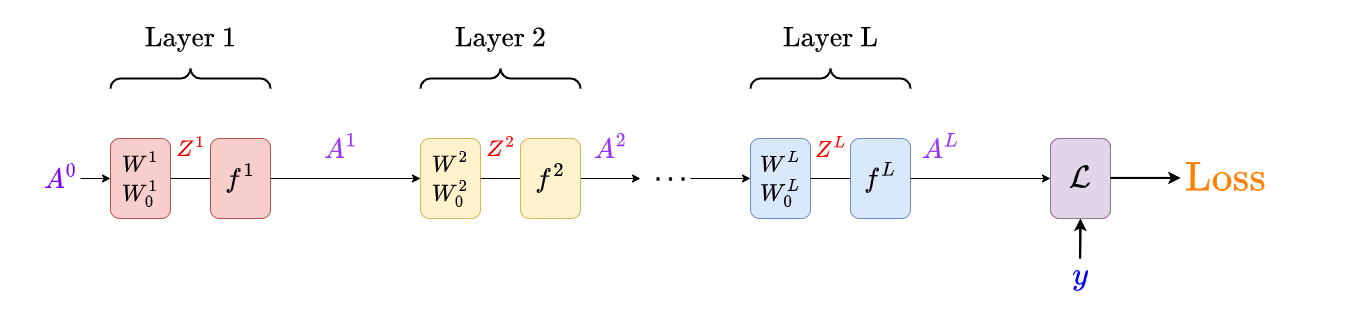
\includegraphics[width=180mm,scale=0.4]{images/nn_1_5_images/network_bp_full.png}
            \caption*{Pretty much the same! Only major difference: swapped scalars for vectors, and vectors for matrices (represented by switching to uppercase)}
        \end{figure}
        
        And, we do backprop the same way, too.
        
        Here, we're not going to explain much as we go: all we're doing is getting the \textbf{derivatives} we need for our \textbf{chain rule}! 
        
        As we go \textbf{backwards}, we can build the gradient for each \textbf{weight} we come across, in the way we described above.
        
        As always, we start from the loss function:
        
        \begin{figure}[H]
            \centering
            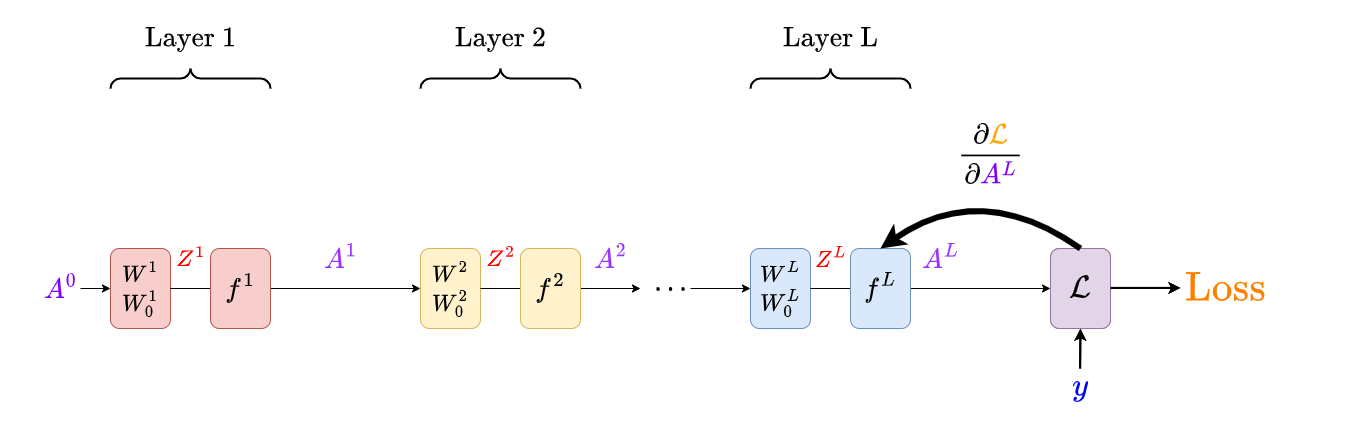
\includegraphics[width=180mm,scale=0.4]{images/nn_1_5_images/network_bp_full1.png}
        \end{figure}
        
        Take another step:
        
        \begin{figure}[H]
            \centering
            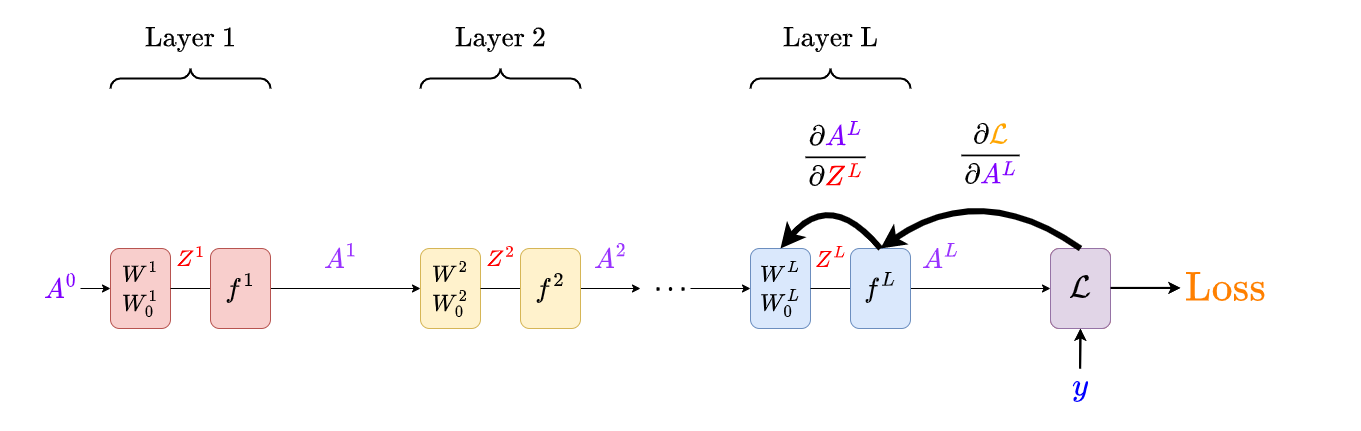
\includegraphics[width=180mm,scale=0.4]{images/nn_1_5_images/network_bp_full2.png}
        \end{figure}
        
        We'll pick up the pace: we'll jump to layer 2 and get its gradient.
            \note{The term $\pderivslash{\red{Z^L}}{\pur{A^2}}$ contains lots of derivatives from every layer between $L$ and 2. \\
            
            But, all we're omitting is the same kinds of steps we're doing in layers 1, 2, and L.}
        
        \begin{figure}[H]
            \centering
            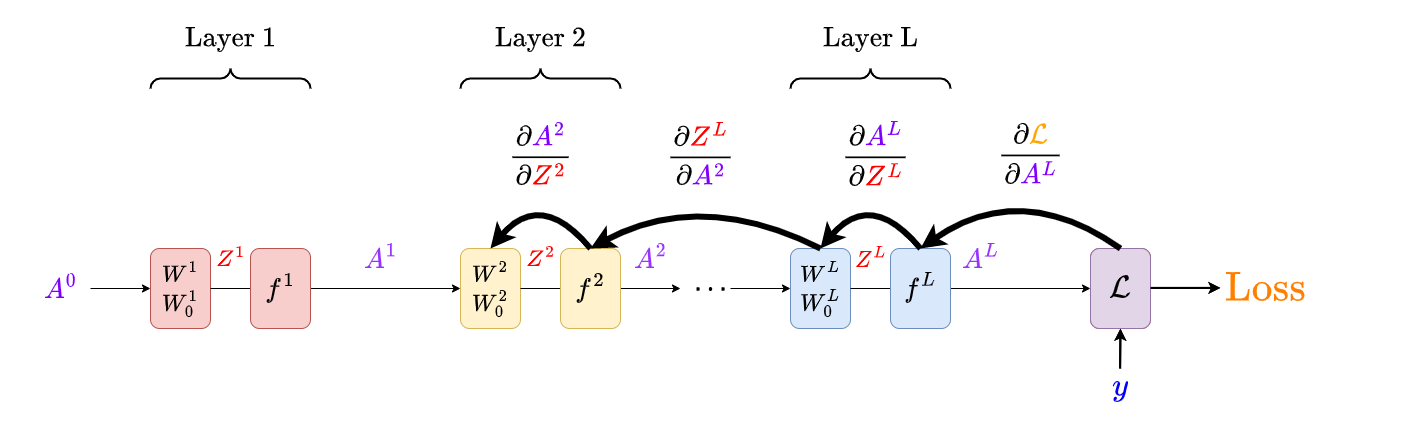
\includegraphics[width=180mm,scale=0.4]{images/nn_1_5_images/network_bp_full3.png}
        \end{figure}
        
        Now, we finally get to layer 1!
        
        \begin{figure}[H]
            \centering
            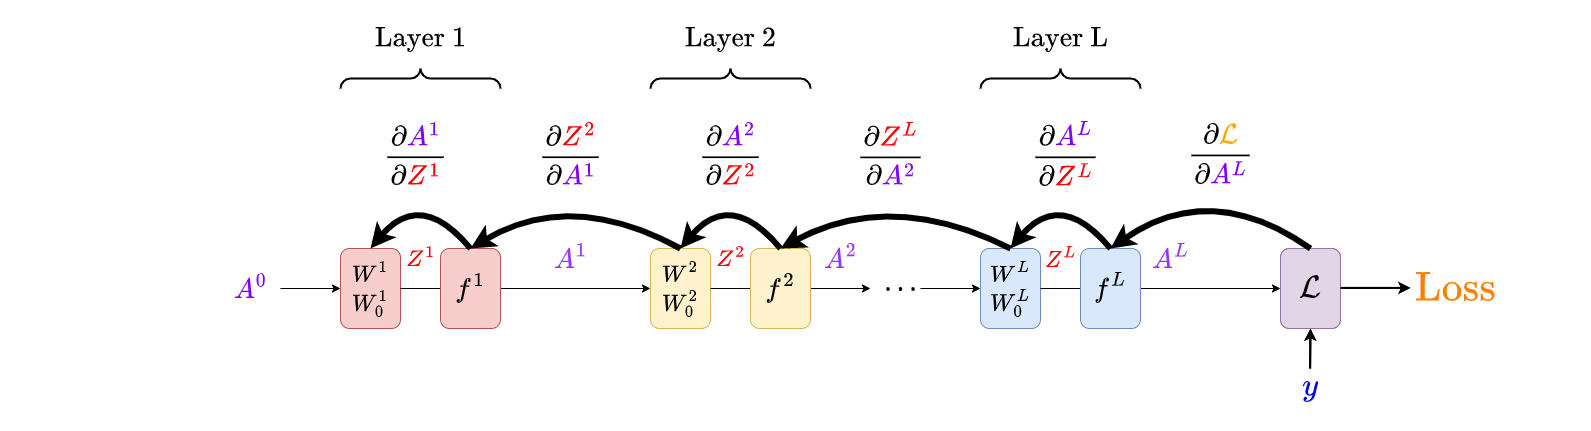
\includegraphics[width=180mm,scale=0.4]{images/nn_1_5_images/network_bp_full4.png}
        \end{figure}
        
        We finish off by getting what we're after: the gradient for $W^1$.\\
        
        \begin{notation}
            We depict neural network gradient descent using the below diagram (outside the box):
            
            The \gren{right}-facing \gren{straight} arrows come \purp{first}: they're part of the \vocab{forward pass}, where we get all of our values.
            
            The \gren{left}-facing \gren{curved} arrows come \purp{after}: they represent the \vocab{back-propagation} of the gradient.
        \end{notation}
        
        \begin{figure}[H]
            \centering
            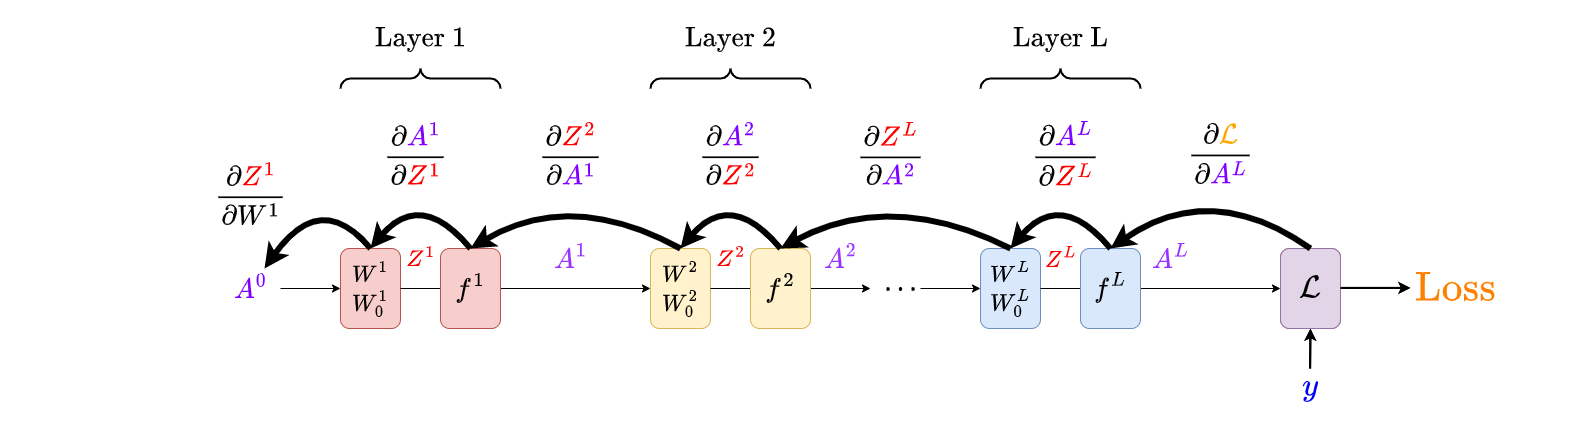
\includegraphics[width=180mm,scale=0.4]{images/nn_1_5_images/network_bp_full5.png}
        \end{figure}
        
        And, with this, we can rewrite our general equation for neural network gradients.
        
    \secdiv
    
    \subsection{How the Chain Rule changes in Matrix form}
        
        As we discussed before, we can't just add onto our weight gradient to reach another layer: the final term
        
        \begin{equation}
            \pderiv{Z^\ell}{W^\ell}
        \end{equation}
        
        Ends our chain rule when we add it: $W^\ell$ isn't part of the input or output, so it doesn't connect to the previous layer.
        
        So, for this section, we'll add it \textbf{separately} at the end of our chain rule:
        
        \begin{equation*}
            \pderiv {\pur{\loss}} {W^\ell} 
            =
            \overbrace{
                \pderiv {\red{Z^\ell}}   {W^{\ell}}
            }^{\text{Weight link}} 
                \cmul
            \overbrace{
                \Bigg(
                    \pderiv {\pur{\loss}} {\red{Z^\ell}}
                \Bigg)^T
            }^{\text{Other layers}}
        \end{equation*}
        
        That way, we can add onto $\pderivslash {\pur{\loss}} {\red{Z^\ell}}$ without worrying about the weight derivative.
            
        Notice two minor changes caused by the switch to matrices:
        
        \begin{itemize}
            \item The order has to be \textbf{reversed}.
            \item We also have to do some weird \textbf{transposing}.
        \end{itemize}
        
        Both of these mostly boil down to trying to be careful about \textbf{shape}/dimension agreement.
            \note{There are also deeper interpretations, but they aren't worth digging into for now.}\\
        
        \begin{notation}
            The \vocab{gradient} $\nabla_{W^\ell} \loss$ for a neural network is given as:
            
            \begin{equation*}
                \pderiv {\pur{\loss}} {W^\ell} 
                =
                \overbrace{
                    \pderiv {\red{Z^\ell}}   {W^{\ell}}
                }^{\text{Weight link}} 
                    \cmul
                \overbrace{
                    \Bigg(
                        \pderiv {\pur{\loss}} {\red{Z^\ell}}
                    \Bigg)^T
                }^{\text{Other layers}}
            \end{equation*}
            
            We get our remaining terms $\pderivslash {\pur{\loss}} {\red{Z^\ell}}$ by our usual chain rule:
            
            \begin{equation*}
                \pderiv {\pur{\loss}} {Z^\ell}
                =
                \overbrace{
                    \Bigg(
                        \pderiv {\blu{A^\ell}}   {\red{Z^\ell}}
                    \Bigg) 
                }^{\text{Layer $\ell$}}
                \cdot
                \Bigg(
                    \cdots 
                \Bigg)
                \cdot
                \overbrace{
                    \Bigg(
                        \pderiv {\red{Z^{L-1}}}   {A^{L-2}}
                            \cmul
                        \pderiv {\blu{A^{L-1}}}   {\red{Z^{L-1}}}
                    \Bigg) 
                }^{\text{Layer $L-1$}}
                \cdot
                \overbrace{
                    \Bigg(
                        \pderiv {\red{Z^L}}   {A^{L-1}}
                            \cmul
                        \pderiv {\blu{A^L}}   {\red{Z^L}}
                    \Bigg) 
                }^{\text{Layer $L$}}
                \cdot
                \overbrace{
                    \Bigg(
                        \pderiv {\pur{\loss}} {\blu{A^L}} 
                    \Bigg)
                }^{\text{Loss unit}}
            \end{equation*}
        \end{notation}
        
        This is likely our most important equation in this chapter!
        
    \secdiv
    
    \subsection{Relevant Derivatives}
    
        If you aren't interesting in understanding matrix derivatives, here we provide the general format of each of the derivatives we care about.\\
        
        \begin{notation}
            Here, we give useful \vocab{derivatives} for \vocab{neural network gradient descent}.
        
            \boxdiv
            
            Loss is not given, so we can't compute it, as before:
            \begin{equation*}
                \overbrace{
                    \pderiv {\pur{\loss}}{\blu{A^L}}
                }^{(n^{L} \times 1)}
            \end{equation*}
            
            \boxdiv
            
            We get the same result for each of these terms as we did before, except in matrix form.
            
            \begin{equation*}
                \overbrace{
                    \pderiv {\red{Z^\ell}}   {W^{\ell}} 
                }^{ (m^{\ell} \times 1) }
                = 
                \blu{A^{\ell-1}}
            \end{equation*}
            
            \begin{equation*}
                \overbrace{
                    \pderiv{\red{Z^\ell}} {\blu{A^{\ell-1}}}
                }^{ (m^{\ell} \times n^{\ell}) }
                =
                W^\ell
            \end{equation*}
            
            \boxdiv
            
            The last one is actually pretty different from before:
            
            \begin{equation*}
                \overbrace{
                    \pderiv {\blu{a^\ell}}   {\red{z^\ell}}
                }^{ (n^{\ell} \times n^{\ell}) }
                =
                \begin{bmatrix}
                    f'({\red{z_1^\ell}})&0                   &0                   &\cdots  & 0 \\
                    0                   &f'({\red{z_2^\ell}})&0                   &\cdots  & 0 \\
                    0                   &0                   &f'({\red{z_3^\ell}})&\cdots  & 0 \\
                    \vdots              &\vdots              &\vdots              &\ddots  & 0 \\
                    0                   &0                   &0                   &0   &f'({\red{z_r^\ell}})
                \end{bmatrix}
            \end{equation*}
            
            Where $r$ is the length of $Z^\ell$.
        \end{notation}
        
        
        
        In short, we only have the $\red{z_i}$ derivative on the $\nth{i}$ diagonal.
            \note{Why this is will be explained in the matrix derivative notes.}
        
        \miniex Suppose you have the activation $f(\red{z}) = \red{z}^2$.
        
        Your pre-activation might be 
        
        \begin{equation}
            \red{z^\ell} = 
            \begin{bmatrix}
                1 \\ 2 \\ 3
            \end{bmatrix}
        \end{equation}
        
        The output would be 
        
        \begin{equation}
            \blu{a^\ell} 
            = 
            f(\red{z^\ell})
            = 
            \begin{bmatrix}
                1 \\ 2^2 \\ 3^2
            \end{bmatrix}
        \end{equation}
        
        But the derivative would be:
        
        \begin{equation}
            f(\red{z}) = 2z
        \end{equation}
        
        Which, gives our matrix derivative as:
        
        \begin{equation*}
            \pderiv {\blu{a^\ell}}   {\red{z^\ell}}
            =
            \begin{bmatrix}
                2\cdot 1 & 0         & 0         \\
                0        & 2 \cdot 2 & 0         \\
                0        & 0         & 2 \cdot 3 \\
            \end{bmatrix}
            =
            \begin{bmatrix}
                2 & 0 & 0  \\
                0 & 4 & 0  \\
                0 & 0 & 6  \\
            \end{bmatrix}
        \end{equation*}
        
        If you want to be able to \textbf{derive} some of the derivatives, without reading the matrix derivative section, just use this formula for vector derivatives:
            \note{If you have time, do read - you won't understand what you're doing otherwise!}
        
        \begin{equation}
                \pderiv{ \pur{w} }{ \org{v} } 
                =
                \overbrace{
                    \begin{bmatrix}
                        \begin{matrix}
                            \bigpderiv{ \pur{w_1} }   { \org{v_1} }\\ 
                            \\
                            \bigpderiv{ \pur{w_1} }   { \org{v_2} }\\ 
                            \\
                            \vdots \\ 
                            \\
                            \bigpderiv{ \pur{w_1} }   { \org{v_m} }
                        \end{matrix} &
                        \begin{matrix}
                            \bigpderiv{ \pur{w_2} }   { \org{v_1} }\\ 
                            \\
                            \bigpderiv{ \pur{w_2} }   { \org{v_2} }\\ 
                            \\
                            \vdots \\ 
                            \\
                            \bigpderiv{ \pur{w_2} }   { \org{v_m} }
                        \end{matrix} &
                        \begin{matrix}
                            \cdots\\\\ \cdots \\\\ \ddots \\\\ \cdots
                        \end{matrix} &
                        \begin{matrix}
                            \bigpderiv{ \pur{w_n} }   { \org{v_1} }\\ 
                            \\
                            \bigpderiv{ \pur{w_n} }   { \org{v_2} }\\ 
                            \\
                            \vdots \\ 
                            \\
                            \bigpderiv{ \pur{w_n} }   { \org{v_m} }
                        \end{matrix}
                    \end{bmatrix}
                }^{ \text{\small Column $j$ matches $\pur{w_j}$} }
                \bigggrB{125pt} \text{\small Row $i$ matches $\org{v_i}$} 
            \end{equation}
            
            We can use this for scalars as well: we just treat them as a vector of length 1.
            
            With some cleverness, you can derive the Scalar/Matrix and Matrix/Scalar derivatives as well.  
                \note{This is contained in the matrix derivatives chapter.}
        
            \secdiv

\pagebreak
        


        
        
\pagebreak
%%%%%%%%%%%%%%%%%%%%%%%%%%%%%%%%%%%%%%%%%%%%%%%%%%%%%%%%%%%%%%%%%%%%%%%%%%%%%  
\section{Training}
    \label{training}
    
    \subsection{Comments}
    
        A few important side notes on training. First, on derivatives:\\
        
        \begin{concept}
            Sometimes, depending on your \purp{loss} and \purp{activation} function, it may be easier to directly compute
            
            \begin{equation*}
                \pderiv{ \pur{\loss} }{ \red{Z}^{L} }
            \end{equation*}
            
            Than it is to find 
            
            \begin{equation*}
                \pderivslash{ \pur{\loss} }{ \org{A}^L } 
                \;\;
                \text{and}
                \;\;
                \pderivslash{ \org{A}^L } { \red{Z}^{L} }
            \end{equation*}
            
            So, our algorithm may change slightly.
        \end{concept}
        
        Another thought: intialization.\\
        
        \begin{concept}
            We typically try to pick a \vocab{random initalization}. This does two things:
            
            \begin{itemize}
                \item Allows us to avoid weird \gren{numerical} and \gren{symmetry} issues that happen when we start with $\blu{W}_{ij}=0$.
                
                \item We can hopefully find different \gren{local minima} if we run our algorithm multiple times.
                    \begin{itemize}
                        \item This is also helped by picking \purp{random data points} in \vocab{SGD} (our typical algorithm).
                    \end{itemize}
            \end{itemize}
            
            Here, we choose our \purp{initialization} from a \gren{Gaussian} distribution, if you know what that is.
        \end{concept}
        
            \note{If you do not know a gaussian distribution, that shouldn't be a problem. It is also known as a "normal" distribution.}

        
    
    \subsection{Pseudocode}
    
        Our training algorithm for backprop can follow smoothly from what we've laid out.
     
        \begin{codebox}
            \Procname{$\proc{SGD-Neural-Net}(\dataTrain, T, L, (m^1, \ldots,
                        m^L), (f^1, \ldots, f^L), \text{Loss})$}
            
            \li \For every \textbf{layer}:
                \Do
                \li \textit{Randomly} initialize
                    \Do
                    \li the \gren{weights} in every layer
                    \li the \gren{biases} in every layer
                    \End
                \End
                \li
            
            \li While \gren{termination condition} not met:
                \Do
                    \li Get random data point \org{$i$}
                    \li Kepp track of time $t$
                    \li
                    \li Do forward pass
                        \Do
                            \li \For every \textbf{layer}:
                                \Do
                                    \li Use previous \textbf{layer}'s \orgg{output}: get \redd{pre-activation}
                                    \li Use \redd{pre-activation}: get new output, \orgg{activation}
                                \End
                                \li
                            
                            \li Get \purp{loss}: forward pass complete
                        \End
                        \li
                    
                    \li Do back-propagation
                        \Do
                            \li \For every \textbf{layer} in \underline{reversed order}:
                            
                            \Do
                                \li If \textbf{final} layer:
                                \gre{\#Loss function}
                                    \Do
                                        \li Get $\pderivslash{ \pur{\loss} }{ \org{A}^L }$
                                    \End
                                    \li
                                
                                \li Else: 
                                    \Do
                                        \li Get $\pderivslash{ \pur{\loss} }{ \org{A^\ell} }$:
                                        \gre{\#Link two layers}
                                            \Do
                                                \li 
                                                $( \pderivslash{ \red{Z}^{\ell+1} }{ \org{A}^\ell } )$ 
                                                \;*\; 
                                                $( \pderivslash{ \pur{\loss} }{ \red{Z}^{\ell+1} } )$ 
                                            \End
                                            \li 
                                             
                                        \li Get $\pderivslash{ \pur{\loss} }{ \red{Z}^{\ell} }$:
                                        \gre{\#Within layer}
                                            \Do
                                                \li
                                                $( \pderivslash{ \org{A}^\ell }{ \red{Z}^{\ell} } )$ 
                                                \;*\;
                                                $( \pderivslash{ \pur{\loss} }{ \org{A}^\ell } )$ 
                                            \End
                                            \li
                                    \End
                                    
                                    
                                \li Compute weight gradients:
                                    \Do
                                        \li Get $\pderivslash{ \pur{\loss} }{ \blu{W}^{\ell} }$:
                                        \gre{\#Weights}
                                            \Do
                                                \li $\pderivslash{\red{Z}^{\ell}}{ \blu{W}^\ell }
                                                = \red{A}^{\ell-1}$
                                                \li
                                                $( \pderivslash{\red{Z}^{\ell}}{ \blu{W}^\ell } )$ 
                                                \;*\;
                                                $( \pderivslash{ \pur{\loss} }{ \red{Z}^{\ell}} )$ 
                                            \End
                                            \li
                                        
                                        \li Get $\pderivslash{ \pur{\loss} }{ \blu{W_0}^{\ell} }$:
                                        \gre{\#Biases}
                                            \Do
                                                \li
                                                $\pderivslash{ \pur{\loss} }{ \blu{W_0}^{\ell} }
                                                =
                                                ( \pderivslash{ \pur{\loss} }{ \red{Z}^{\ell}} )$ 
                                            \End
                                            \li
                                    \End
                                    
                                \li Follow Stochastic Gradient Descend (SGD): \gre{\#Take step}
                                    \Do   
                                        \li Update \gren{weights}:
                                        \Do
                                            \li $\blu{W}^\ell = \blu{W}^\ell - 
                                            \Big( \eta(t) * (\pderivslash{ \pur{\loss} }{ \blu{W}^{\ell} }) \Big)$
                                        \End
                                        \li
                                        
                                        \li Update \gren{biases}:
                                        \Do
                                            \li $\blu{W_0}^{\ell} = \blu{W_0}^{\ell} - 
                                            \Big( \eta(t) * (\pderivslash{ \pur{\loss} }{ \blu{W_0}^{\ell} }) \Big)$
                                        \End
                                        
                                        \li
                                        
                                    \End
                            \End
                        \End

                \End
            \li Return final neural network with weights and biases
    
        \end{codebox}
\pagebreak
%%%%%%%%%%%%%%%%%%%%%%%%%%%%%%%%%%%%%%%%%%%%%%%%%%%%%%%%%%%%%%%%%%%%%%%%%%%%%  

\section*{Terms}
    
    \begin{itemize}
        \item Forward pass
        \item Back-Propagation
        \item Weight gradient
        \item Matrix Derivative
        \item Partial Derivative
        \item Multivariable Chain Rule
        \item Total Derivative
        \item Size of a matrix
        \item Planar Approximation
        \item Scalar/scalar derivative
        \item Vector/scalar derivative
        \item Scalar/vector derivative
        \item Vector/vector derivative
        
    \end{itemize}